\documentclass[tikz,border=8pt]{standalone}
\begin{document}
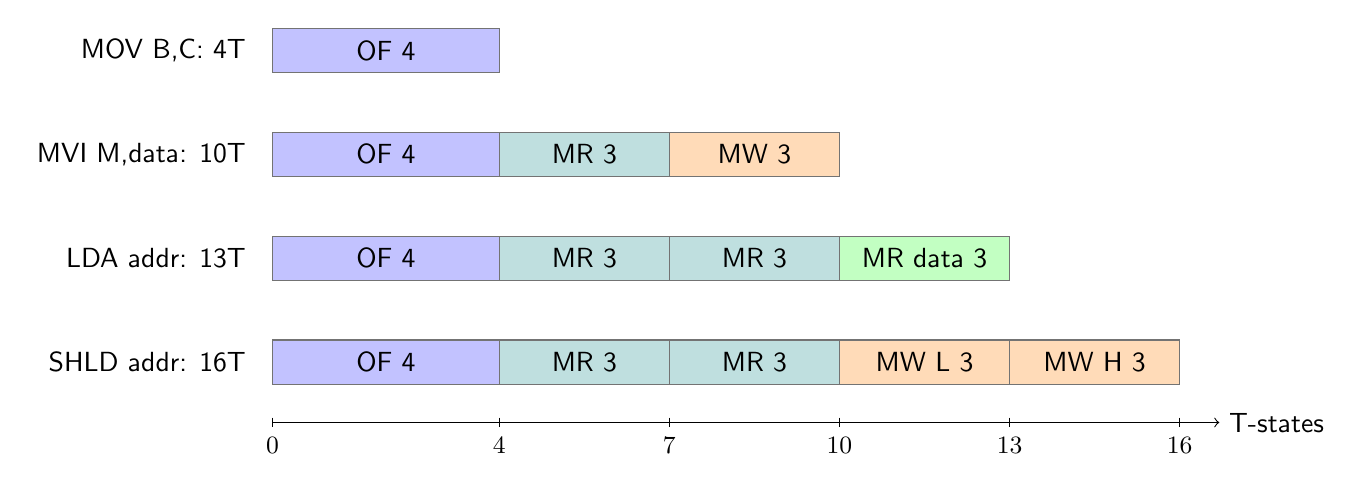
\begin{tikzpicture}[font=\sffamily,x=0.72cm,y=0.88cm]
\def\cy#1#2#3#4{\draw[fill=#4,draw=black!55] (#1,#2) rectangle ++(#3,.64);}
\foreach \y/\lab in {4.5/{MOV B,C: 4T},3/{MVI M,data: 10T},1.5/{LDA addr: 13T},0/{SHLD addr: 16T}}{\node[anchor=east] at (-.3,\y+.32){\lab};}
\cy{0}{4.5}{4}{blue!24}\node at (2,4.82){OF 4};
\cy{0}{3}{4}{blue!24}\node at (2,3.32){OF 4};\cy{4}{3}{3}{teal!25}\node at (5.5,3.32){MR 3};\cy{7}{3}{3}{orange!28}\node at (8.5,3.32){MW 3};
\cy{0}{1.5}{4}{blue!24}\node at (2,1.82){OF 4};\cy{4}{1.5}{3}{teal!25}\node at (5.5,1.82){MR 3};\cy{7}{1.5}{3}{teal!25}\node at (8.5,1.82){MR 3};\cy{10}{1.5}{3}{green!24}\node at (11.5,1.82){MR data 3};
\cy{0}{0}{4}{blue!24}\node at (2,.32){OF 4};\cy{4}{0}{3}{teal!25}\node at (5.5,.32){MR 3};\cy{7}{0}{3}{teal!25}\node at (8.5,.32){MR 3};\cy{10}{0}{3}{orange!28}\node at (11.5,.32){MW L 3};\cy{13}{0}{3}{orange!28}\node at (14.5,.32){MW H 3};
\draw[->] (0,-.55)--(16.7,-.55) node[right]{T-states};
\foreach \x in {0,4,7,10,13,16}{\draw (\x,-.48)--(\x,-.62) node[below,font=\small]{\x};}
\end{tikzpicture}
\end{document}
